\chapter{The Mindset Behind an Unforgettable Novel}

This lecture is an interview rather than a board lecture, so its rigor is not symbolic in the usual sense. It is procedural, comparative, and architectural. The first half-minute is an overture rather than the true beginning: we hear, in compressed form, the lecture's eventual claims about readerly presence, outlining, poetic surprise, and the feedback loop of description. Then the conversation resets and begins where the host actually begins, with admiration for Amor Towles's descriptive precision and vocabulary. Because no validated board images survive for this lecture, the displayed relations and diagrams below are cautious transcript-based reconstructions rather than transcriptions of visible equations. The conversation between David Perell and Amor Towles belongs to the curated LazyingArt LLC collection \emph{How You Speak and Write}.

\section{Prelude, Vocabularies, and Social Worlds}

The lecture's first real movement begins not with plot, pacing, or symbolism, but with vocabulary. Perell notices Towles's socially precise language, and in particular the French-inflected diction of \emph{A Gentleman in Moscow}. Towles immediately widens the category. A writer, he says, becomes interested in vocabularies of every kind: baseball, city streets, finance, ethnic neighborhoods, technical disciplines, even the language of physics. The point is not lexical display. The point is that different situations demand different verbal pressures, and the writer slowly trains his ear to hear them.

This is why the Count is the right opening example. Count Rostov is an aristocrat formed in late nineteenth-century Europe. French therefore belongs to his world; it is not decoration. Towles sharpens the point by admitting that he himself does not speak French fluently. What matters is not exhaustive mastery but the accurate evocation of social sensibility. A few strategically chosen elements can bring into focus the class, education, and habits of a man for whom French-inflected speech would be natural.

From there the conversation broadens to a second contrast. If \emph{A Gentleman in Moscow} draws on aristocratic and European registers, \emph{The Lincoln Highway} must sound like midcentury America. To prepare that soundscape, Towles returns to several American books written around the same historical moment. The exact bibliographic sequence in the transcript is somewhat unstable, but the argument is clear: books written within roughly the same period can still carry radically different vocabularies, concerns, and tonalities while remaining unmistakably American. Language is not merely a sign of talent. It is a way of choosing a world.

\subsection{Question \& Answer}

\paragraph{How do we use a language-world that we only partly possess ourselves?}

Towles's answer is modest and practical. We do not wait for perfect mastery. We listen, absorb, and gather fragments that carry real social pressure. Then, when we write, we use those fragments to evoke sensibility rather than to prove authority. The standard is not encyclopedic control. The standard is that the chosen language belongs to the character's world.

\section{Readerly Presence and the Economy of Description}

Perell's transition into Towles's essay on Hopper's \emph{Nighthawks} shifts the lecture from vocabulary to effect. He describes the experience of encountering a mood he had not previously named. Towles responds by identifying the deeper aim. One of the most important things, he says, is to make the reader feel that he is living the experience in the book. Description matters because it is one of the chief means by which that state is achieved.

\begin{definition}
By \emph{readerly presence} we mean the condition in which the reader feels located inside the scene, can orient himself within it, and can therefore become interested in the thoughts, feelings, and actions unfolding there.
\end{definition}

Towles's causal chain is explicit enough that we may safely render it schematically:
\begin{equation}
\text{description} \longrightarrow \text{readerly presence} \longrightarrow \text{readerly engagement}.
\end{equation}
This is not literal lecture mathematics. It is a compact notation for a spoken claim. Description is valuable because it helps the reader feel present, and presence is what allows connection to character and event.

The hotel in \emph{A Gentleman in Moscow} supplies the model case. Because the novel remains inside that environment for decades, Towles knows that the geography of the hotel must be established early. Key rooms must become vivid early. Once that orientation is in place, later movement through the building will feel natural rather than arbitrary.

A second relation follows:
\begin{align}
\text{too little detail} &\Rightarrow \text{weak presence}, \\
\text{too much detail} &\Rightarrow \text{drag}, \\
\text{effective description} &\text{ lies in the narrow middle region.}
\end{align}
The transcript is badly garbled at precisely this point, but the underlying argument is firm. Description cannot be so sparse that the scene could be anywhere, and it cannot be so specific and cumbersome that the reader becomes trapped in cold inventory. The writer adds and removes detail until he finds the few elements that make the space come alive.

\begin{figure}[h]
\centering
\begin{tikzpicture}[>=stealth]
\node[draw, rectangle, minimum width=3.0cm, minimum height=0.9cm] (a) at (0,0) {Describe};
\node[draw, rectangle, minimum width=3.0cm, minimum height=0.9cm] (b) at (4.0,0) {See More};
\node[draw, rectangle, minimum width=3.6cm, minimum height=0.9cm] (c) at (8.6,0) {Describe More};
\draw[->] (a) -- (b);
\draw[->] (b) -- (c);
\draw[->] (c) to[out=35,in=145] (a);
\end{tikzpicture}
\caption{Transcript-based schematic reconstruction of Towles's iterative loop. Description sharpens perception, and sharpened perception returns to language.}
\end{figure}

The overture at the beginning of the lecture announces this loop before the conversation has properly started, and later Towles states it directly:
\begin{equation}
\text{describe} \longrightarrow \text{see more} \longrightarrow \text{describe more}.
\end{equation}
The crucial point is that description is not mere report. Once we begin to describe, we begin to notice more; once we notice more, language can deepen.

\subsection{Question \& Answer}

\paragraph{How much description is enough to make a place vivid without bogging the reader down?}

Enough to orient the reader, not enough to imprison him. The writer does not aim at exhaustive totality. He aims at the details that let the reader know where he is, move through the space, and feel events taking place there. In practice this means writing, rereading, adding, subtracting, and discovering which details are actually doing the work.

\section{Pacing, Editing, and Urgency Without Action}

From the balance of description the lecture turns naturally to tempo. Perell asks how one judges pacing when repeated exposure distorts one's own sense of it. Towles answers by renaming the subject. What Perell is really asking about, he says, is editing.

Writing and editing are closely interlinked, but they are not the same skill. Editing means returning to what one has already written and hearing it with a colder ear. Towles gives a blunt criterion: if a section feels boring to him on rereading, that is already a warning sign. The reader is even more at risk.

The key clarification is that pace is not the same thing as page-turning action:
\begin{equation}
\text{urgency} \neq \text{action}.
\end{equation}
A classical page-turner is driven by crisis, danger, and event. That is one art form. Literary urgency is broader. A reader may be drawn forward by curiosity about a character's psychology, by tonal pressure, by the compulsion of a sentence, or by the desire to understand what a mind will do next, even when outward action is minimal.

This distinction preserves a freedom that many discussions of pacing destroy. A literary novel may contain slow passages. What matters is whether the slowness is alive. If the prose continues to generate inward motion, then the reader is still being carried.

\subsection{Question \& Answer}

\paragraph{How can a novel create urgency when little external action is occurring?}

By making continuation necessary. The reader can be compelled forward by psychology, phrasing, tonal pressure, or an unresolved question. This is why Towles insists that the target is not simply speed. It is momentum.

\section{Premise, Scaffolding, and Freeing the Poetic Mind}

After the discussion of pacing, Towles steps back and describes the architecture of his process. This is one of the lecture's most formal passages. His novels begin, he says, with a very simple premise, often a single sentence. In the case of \emph{A Gentleman in Moscow}, the premise is something like a man living in a hotel for a long period of time. If the premise has force, it expands rapidly. The setting, social identity, political constraint, and historical span appear almost at once.

We may summarize the pipeline as
\begin{equation}
\text{premise} \longrightarrow \text{rapid expansion} \longrightarrow \text{scaffolding} \longrightarrow \text{notebooks} \longrightarrow \text{draft} \longrightarrow \text{revision}.
\end{equation}

Towles is unusually specific about timing:
\begin{enumerate}
\item In about \(1.5\) hours, he wrote down the key elements of \emph{A Gentleman in Moscow}.
\item In roughly \(3\) days, he wrote the scaffolding for most of the key events.
\item Over a couple of years, he filled notebooks with scene investigations and visualized moments.
\item Only then did he write the book itself, over about \(1.5\) years.
\item After that came \(2\) or \(3\) revision passes from beginning to end.
\end{enumerate}

\begin{figure}[h]
\centering
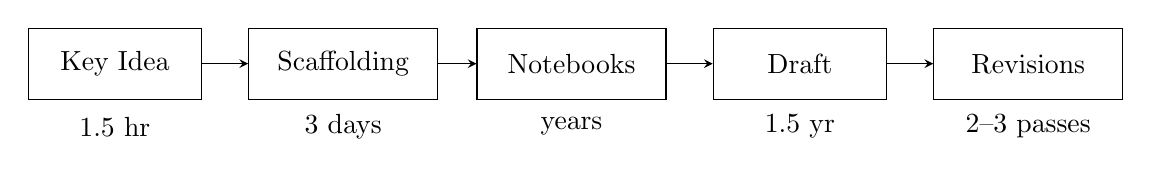
\begin{tikzpicture}[>=stealth]
\node[draw, rectangle, minimum width=2.2cm, minimum height=0.9cm] (a) at (0,0) {Key Idea};
\node[draw, rectangle, minimum width=2.4cm, minimum height=0.9cm] (b) at (2.9,0) {Scaffolding};
\node[draw, rectangle, minimum width=2.4cm, minimum height=0.9cm] (c) at (5.8,0) {Notebooks};
\node[draw, rectangle, minimum width=2.2cm, minimum height=0.9cm] (d) at (8.7,0) {Draft};
\node[draw, rectangle, minimum width=2.4cm, minimum height=0.9cm] (e) at (11.6,0) {Revisions};
\draw[->] (a) -- (b);
\draw[->] (b) -- (c);
\draw[->] (c) -- (d);
\draw[->] (d) -- (e);
\node at (0,-0.8) {$1.5$ hr};
\node at (2.9,-0.8) {$3$ days};
\node at (5.8,-0.8) {years};
\node at (8.7,-0.8) {$1.5$ yr};
\node at (11.6,-0.8) {$2$--$3$ passes};
\end{tikzpicture}
\caption{Transcript-based schematic reconstruction of Towles's process. The striking feature is not merely the sequence, but how much structural work is done before chapter one is drafted.}
\end{figure}

The notebooks matter because they remove live uncertainty from the drafting stage. Towles is not sitting before a blank page trying to solve, in real time, where the room is, who is present, what the emotional context is, and what event should occur. Much of that has already been precomputed. The drafting question becomes a better question: what is the best language for bringing this already imagined scene to life?

This leads to the lecture's most memorable process relation:
\begin{equation}
\text{more precomputed structure} \Rightarrow \text{less analytic load} \Rightarrow \text{more poetic freedom}.
\end{equation}
Towles expresses the point with the familiar left-brain/right-brain metaphor. We should take that language as heuristic rather than neuroscientific. The argument itself is clear. If the problem-solving side of the mind must stay fully engaged during drafting, then the more dreamlike and poetic side is damped down. Planning is therefore not the enemy of surprise. It is one of the conditions under which surprise becomes possible.

\subsection{Question \& Answer}

\paragraph{Why plan so much if what we want in the end is spontaneity and discovery?}

Because Towles's spontaneity is not the spontaneity of uncertainty. It is the spontaneity that becomes possible once structural burdens have been lifted. Planning does not replace surprise. It creates the space in which surprise can enter the sentence.

\section{Point of View, Symbolism, and Character-Conscious Detail}

The next local obstacle is symbolism, though the host's prompt in the transcript is badly corrupted. Towles's answer is clear. He does not begin with symbols as detachable ornaments. He begins with narration.

\emph{A Gentleman in Moscow} is written in the third person, but not in the fully omniscient mode of Dickens, Tolstoy, or Henry James. The distinction may be expressed schematically as
\begin{equation}
K_{\text{close third}} \subset K_{\text{omniscient third}}.
\end{equation}
An omniscient narrator knows the whole field: all pasts, futures, and inner lives. Towles's narration stays much closer to the Count. It tells us what he would notice, in tones he would plausibly feel, with comic and social inflections that belong to his consciousness.

This is why a resonant detail is not, in the first instance, a matter of symbolic insertion. It is often the consequence of asking a narrower and better question. Not \emph{How shall we describe the coffee?} but \emph{What would the Count notice about the coffee?} Towles's answer is telling. The Count notices service, promptness, temperature, cuisine, and the dignity of things done well. Those are not arbitrary observations. They arise from aristocratic habit, temperament, value, and humor.

One of the strongest claims in the lecture follows from this. Many of the passages readers later call moving or beautiful were not sentences Towles would naturally say in his own life. They were sentences discovered by inhabiting another consciousness deeply enough that the language seemed to come from that person. The joking line ``Well done, Count'' reveals the structure of the experience. When the voice is alive, the sentence arrives as if from within the character's world.

Before the lecture returns to description through a full example, it makes a brief but revealing digression. Towles rejects the glamorous myth of the chaotic artist and describes writing instead as regular work. Most accomplished writers, he says, punch the clock. Inspiration comes at the desk, not before it. That practical claim matters here because it shows the background condition of all the techniques under discussion: the vivid sentence is not a magical exemption from discipline.

\subsection{Question \& Answer}

\paragraph{Where does symbolism come from if it is not inserted mechanically from above?}

From point of view. Once narration is genuinely attached to a consciousness, the things that become visible in the prose are already charged by temperament, memory, class, value, and feeling. Symbolic force often emerges there, as a byproduct of inhabited perception rather than as a separate layer applied from outside.

\section{The Child in the Kitchen and Revision for the Reader}

Perell now returns to description by way of a deliberately exaggerated image. He suggests, rhetorically, that ordinary perception might get us to ``100,'' while a writer like David Foster Wallace pushes us to ``500.'' Towles does not adopt the number scheme as his own, but he does accept the underlying intuition: good description changes seeing. That is what prepares the lecture's most analytic example.

The scene is simple. A young girl comes downstairs in the early 1960s, enters the kitchen, and sees her mother making dinner. Towles begins by rejecting the obvious mistake. A weak writer, given period reference material, might load the sentence with stock markers: Birdseye peas, Frigidaire, Beatles on the radio. All of that may be historically accurate, and all of it may still be dead. The problem is not falsehood. The problem is that this is not what the child would notice. It is what an outside observer, anxious to signal ``1964,'' would choose.

Towles therefore replaces period labeling with focal perception. What would a seven- or eight-year-old actually see? In his answer, the vivid object is not the brand name but the strange brick of frozen peas sliding out of the package, breaking over the pot, scattering across the counter, perhaps leading the child to taste a frozen pea and discover its peculiar texture. Historical specificity is recovered through consciousness rather than through cliche.

\paragraph{Worked example.}

We hold the overt scene fixed:
\begin{equation}
S = \text{child enters the kitchen at dinner time}.
\end{equation}
Now we vary the hidden state:
\begin{align}
H_1 &= \text{the mother has just discovered her husband's infidelity}, \\
H_2 &= \text{the mother has just committed her own infidelity}.
\end{align}
The visible room may remain almost unchanged, but the realized prose cannot:
\begin{align}
S + H_1 &\Rightarrow D_1, \\
S + H_2 &\Rightarrow D_2, \\
D_1 &\neq D_2.
\end{align}
Here \(D_1\) and \(D_2\) differ not because furniture has moved, but because diction, tempo, gesture, and atmosphere have changed.

\begin{figure}[h]
\centering
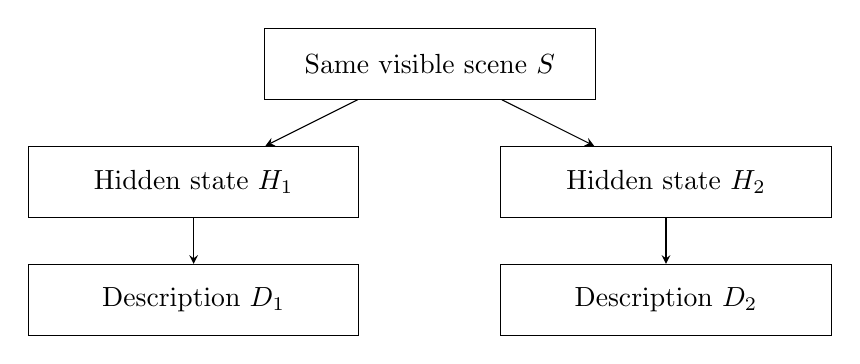
\begin{tikzpicture}[>=stealth]
\node[draw, rectangle, minimum width=4.2cm, minimum height=0.9cm] (s) at (0,2.0) {Same visible scene $S$};
\node[draw, rectangle, minimum width=4.2cm, minimum height=0.9cm] (h1) at (-3.0,0.5) {Hidden state $H_1$};
\node[draw, rectangle, minimum width=4.2cm, minimum height=0.9cm] (h2) at (3.0,0.5) {Hidden state $H_2$};
\node[draw, rectangle, minimum width=4.2cm, minimum height=0.9cm] (d1) at (-3.0,-1.0) {Description $D_1$};
\node[draw, rectangle, minimum width=4.2cm, minimum height=0.9cm] (d2) at (3.0,-1.0) {Description $D_2$};
\draw[->] (s) -- (h1);
\draw[->] (s) -- (h2);
\draw[->] (h1) -- (d1);
\draw[->] (h2) -- (d2);
\end{tikzpicture}
\caption{Transcript-based schematic reconstruction of the kitchen scene. The overt scene can remain fixed while the mother's hidden history changes tone, pace, and language.}
\end{figure}

Towles's point is subtler still. The child may not consciously know what has happened. Yet the mother's behavior must carry the trace of that hidden state, so that later, when the truth is discovered, the reader can return and say: it was all there. The scene was already vibrating with knowledge that the focal consciousness could sense without interpreting.

The lecture's iterative logic returns here with greater force. We begin by observing accurately. Then we choose words. Then we revise toward a larger truth that includes not only what is visible, but the emotional field of the household, the class setting, the regional context, and the historical moment. The scene is not merely a kitchen. It is this kitchen, in this family, under these pressures.

\subsection{Question \& Answer}

\paragraph{How do we avoid cliche and still make a scene historically specific and emotionally loaded?}

By refusing to write like a historian labeling the decade. We ask instead what this perceiver, at this age and in this situation, would actually notice. Then we allow hidden state to reshape the scene's language and tempo from underneath. Historical specificity enters through lived perception, not through a pile of expected markers.

Towles then turns this example into an ethics of drafting. The first draft, he says, is written for himself alone. He lets fascinations, digressions, vanities, and odd pleasures proliferate without restraint. Only later does he reverse the lens and read from the reader's side of the covenant:
\begin{equation}
\text{first draft for self} \longrightarrow \text{revision for reader}.
\end{equation}
That second phase is not a marketing exercise. It is an obligation. If the reader is giving money and, more importantly, time, the writer owes economy in return. Redundancy, boredom, cliche, and purely private indulgence must be cut. Revision is therefore largely subtractive. It makes the prose leaner, sharper, and truer to the story's actual needs. At this stage Towles also turns to a small circle of thoughtful readers, including editors and trusted literary friends, whose responses help him test the book from the outside.

\subsection{Question \& Answer}

\paragraph{What exactly changes when we revise for the reader rather than for ourselves?}

The axis of judgment changes. In the first draft, we allow private fascination to expand. In revision, we ask what belongs to the story and what merely flatters the writer's whim. The result is a movement from abundance to economy, from self-directed exploration to reader-centered form.

\section{Craft, Reading, Poetry, Manifestos, Doors, and New York}

From revision the lecture broadens into teachability. Towles resists speaking as a formal teacher, but his answer is still precise. Much can be taught if by teaching we mean repeated practice, disciplined exposure, and growing command over the elements of craft. He explicitly names a long list:
\begin{itemize}
\item plot,
\item setting,
\item dialogue,
\item tone of voice,
\item perspective,
\item metaphor,
\item simile,
\item allusion,
\item allegory.
\end{itemize}
The decisive word is not genius but repetition. One gains command by writing again and again, and Towles adds an important further demand: young writers should write from many perspectives. Different genders, classes, ages, regions, countries, and sensibilities force the writer to rediscover craft as variable rather than fixed. There is no single formula for ``how to describe a room,'' because the room changes with the mind that enters it.

The same principle governs reading. Towles describes reading and writing as nearly simultaneous from childhood onward. He remembers a first-grade teacher bringing a poet into the classroom and the experience of receiving signed books. That memory matters because it joins language, performance, and authorship at the moment of origin. Later, reading becomes more analytic. He reads with a pen. He studies structure. He writes about structure. He joins a reading group that treats books comparatively and historically. The point is not passive admiration. It is investigation.

A revealing heuristic appears here. History, Towles says, is poor at preserving everything that is great, but comparatively good at discarding what is mediocre. In shorthand form,
\begin{equation}
\text{corpus at } t \longrightarrow \text{filtered canon at } t+50.
\end{equation}
This is a rule of thumb, not a law. But it explains why he and his friends often read older authors: not because the past captured every greatness, but because time has already done some filtering.

Towles also lingers at the sentence level. A paragraph by Roth may move, almost invisibly, from one consciousness to another, or briefly into omniscience, without rupture. That kind of fluid viewpoint movement is powerful precisely because it is dangerous. Mishandled, it jars the reader. Handled well, it enlarges narrative possibility.

His remarks on poetry return to the problem of balance. Too much poetic indeterminacy, sustained without relief, will exhaust the reader. A novel must therefore know when to stabilize orientation and when to let language move toward dream, ambiguity, or resonance. The same balance returns, in another register, in his remarks on manifestos. What interests him is not doctrine as such, but verbal energy. Manifestos are declarative, staccato, self-assured, and action-oriented. They do not slow themselves down with too much explanation:
\begin{equation}
\text{high declaration density} + \text{low explanatory drag} \Rightarrow \text{manifesto energy}.
\end{equation}

The lecture's final metaphor gathers these late themes into a single test. A promising idea is one that opens doors. The writer sees one small thing, or has one compressed premise, and immediately many rooms begin to appear:
\begin{equation}
\text{premise} \Rightarrow \text{many possible continuations}.
\end{equation}
That metaphor allows the conversation to close on New York. For Towles, New York is not merely a melting pot of ethnicity or nationality. It is a melting pot of passions. Journalism, cuisine, dance, finance, law, advertising, theatre, and other pursuits all draw ambitious young people into the same city. The result is a density of overlapping aspiration. That density gives the city its strange electricity, and it explains why New York functions, in Towles's imagination, not only as a setting but as an engine of narrative possibility.

\subsection{Question \& Answer}

\paragraph{What makes an idea rich enough to grow into a novel rather than remain a passing observation?}

Towles's test is branching power. A good premise begins opening rooms almost immediately. If one idea quickly suggests many scenes, many pressures, many characters, and many routes forward, then the writer feels its richness before he has fully written any of it down.

\section{Summary}

This lecture contains no literal board mathematics, yet it is rigorous in a very useful way. It gives us a chain of necessities. Vocabulary must belong to a world. Description must create presence. Presence must support engagement. Editing must distinguish urgency from mere speed. Planning must reduce analytic burden so that surprise can occur inside the sentence. Point of view must generate meaningful detail from within consciousness. Revision must convert private abundance into readerly economy. And reading, finally, must become a reciprocal apprenticeship in which structure, tone, sentence movement, and historical judgment continually return to the writer's own practice.

If we keep the lecture's order in mind, the whole discussion hangs together. It opens with language, narrows to presence, turns to pacing, widens to process, drills down into point of view, reenters the scene through the kitchen example, and then opens outward again into revision, teachability, reading, poetry, manifestos, door-opening premises, and the urban ecology of New York. The result is not a doctrine of inspiration. It is a disciplined account of how imaginative freedom is built.